% !TEX program = xelatex
\documentclass[a4paper]{article}
\usepackage{amsmath}
\usepackage{amsthm}
\usepackage[left=1.8cm,right=1.8cm,top=2.2cm,bottom=2.0cm]{geometry}
\usepackage{ctex}
\usepackage{enumerate}
\usepackage{fancyhdr}
\usepackage{xpatch}
\usepackage{graphicx} 
\usepackage{float} 
\usepackage{subfigure} 
\usepackage{amsfonts}
\usepackage{mathtools}
\usepackage{framed}
\usepackage{multicol}
\usepackage{listings}
\usepackage{hyperref}
\usepackage{listings}
\usepackage{tikz}
\usetikzlibrary{automata,positioning}
\theoremstyle{definition}
\newtheorem*{solution*}{\textbf{Solution:}}
\newtheorem*{proof*}{\textbf{Proof:}}
\newtheorem{theorem}{Theorem}[subsection]
\newtheorem{definition}{Definition}[subsection]
\newtheorem{lemma}{Lemma}[subsection]
\makeatletter

\AtBeginDocument{\xpatchcmd{\@thm}{\thm@headpunct{.}}{\thm@headpunct{}}{}{}}
\makeatother

\pagestyle{fancy}
\renewcommand{\baselinestretch}{1.15}

\usepackage{paralist}
\let\itemize\compactitem
\let\enditemize\endcompactitem
\let\enumerate\compactenum
\let\endenumerate\endcompactenum
\let\description\compactdesc
\let\enddescription\endcompactdesc

% shorten footnote rule
\xpatchcmd\footnoterule
  {.4\columnwidth}
  {1in}
  {}{\fail}

\title{CS 131 Compilers: Discussion 2: (Non)Deterministic Finite Automata}
\author{\textbf{杨易为}~~\textbf{季杨彪}~~\textbf{尤存翰} \\ \texttt{ \{yangyw,jiyb,youch\}@shanghaitech.edu.cn}}



\begin{document}
\maketitle
\section{DFA and NFA}
\subsection{Introduction}

Finite state automata (FSA) are abstract machines that feature states and guarded tran-sitions from one state to another.  An FSA can only be in one state a time, and its totalnumber of states isfinite.  The machine takes transitions in response to inputs it receivessequentially;  if an input matches the guard of a transition that departs from the currentstate that transition is said to be enabled; only enabled transitions can be taken.  FSA thathave an accepting state provide the machinery to determine whether an input string is in aregular language.  If no transitions are enabled by a given input then the entire input stringgets  rejected.   If  all  inputs  are  processed  and  the  FSA  is  in  an  accepting  state  then  theentire input string is accepted.  Deterministic finite state automata (DFA) can only haveone enabled transition at a time while a non-deterministic finite state automata (NFA) canhave multiple.
\\
Before NLP, we utilize state machine to accept languages. Two different perspectives can be considered, namely symbolic and random. chomsky's formal language theory embodies a symbolic approach. Based on this view, a language contains a sequence of symbols that must follow the syntactic rules of its generative grammar. This view reduces the structure of a language to a set of well-defined rules that allow for the decomposition of each sentence and word into structural components.
\subsection{Examples of accepting x86 Assembly}
https://github.com/yangminz/bcst\_csapp
\\
There are three main types of terminators for assembly instructions: Immediately and Scale for numbers, Reg and Op for characters, and other symbols, including spaces (' '), commas (','), and parentheses ('(',')'). For numeric terminators, we can use Deterministic Finite Automation (DFA) to determine and parse them according to Regular Grammar, see below Figure. It should be noted that the numbers in assembly instructions include positive and negative integers in hexadecimal and decimal, and We need to check whether the value overflows at each state transfer step.

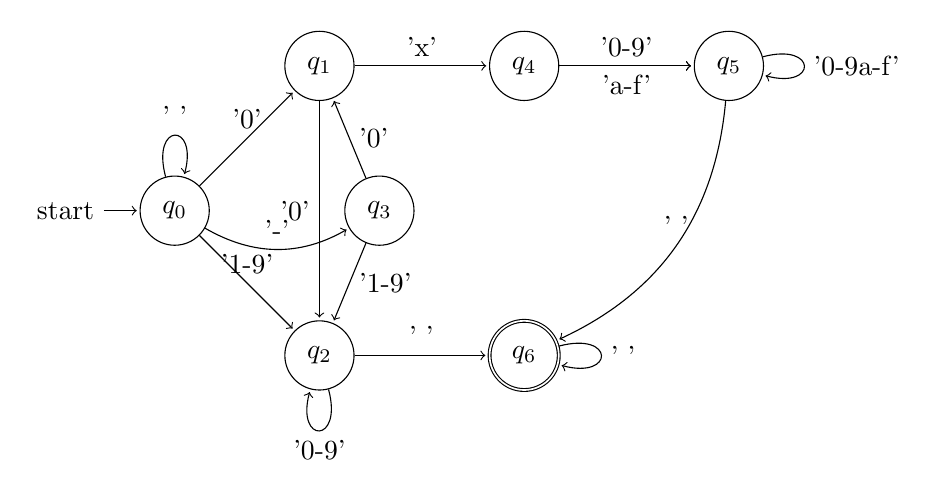
\begin{tikzpicture}[shorten >=1pt,node distance=2.6cm,on grid,auto]
    \node[state,initial] (q_0)   {$q_0$};
    \node[state] (q_1) [ above right=of q_0] {$q_1$};
    \node[state] (q_2) [below right=of q_0] {$q_2$};
    \node[state] (q_3) [ right=of q_0] {$q_3$};
    \node[state] (q_4) [ right=of q_1] {$q_4$};
    \node[state] (q_5) [ right=of q_4] {$q_5$};
    \node[state,accepting] (q_6) [ right=of q_2] {$q_6$};
    \path[->]
    (q_0) edge [loop above] node {' '} ()
        edge  node  [above]{'0'} (q_1)
        edge [bend right] node  [above]{'-'} (q_3)
        edge  node  [above]{'1-9'} (q_2)
    (q_1) edge  node  {'x'} (q_4)
        edge node [left] {'0'} (q_2)
    (q_2) edge  node  {' '} (q_6)
    edge [loop below] node {'0-9'} ()
    (q_3)edge  node [right] {'0'} (q_1)
    edge  node [right] {'1-9'} (q_2)
    (q_4)edge  node  {'0-9'} (q_5)
    edge [below] node  {'a-f'} (q_5)
    (q_5) edge [loop right] node {'0-9a-f'} ()
    edge [bend left] node [above] {' '} (q_6)
    (q_6) edge [loop right] node {' '} ()
        ;

\end{tikzpicture}\\
For character type terminators, i.e. operands and registers, we can take a simple string matching (Matching). Here, we have a variety of data structures to employ. The most common approach is to use an array or list that stores all possible string values, e.g., \{"rax","eax"\} and \{"mov","ld","sd"\}, and iterate through this array and match each element. With such a data structure, the time complexity of finding and matching is $O(LE[strlen])$, where $E[strlen]$ is the average length of the string. Another strategy is to build a dictionary tree (Trie) or a prefix tree for the above array of strings.
\\
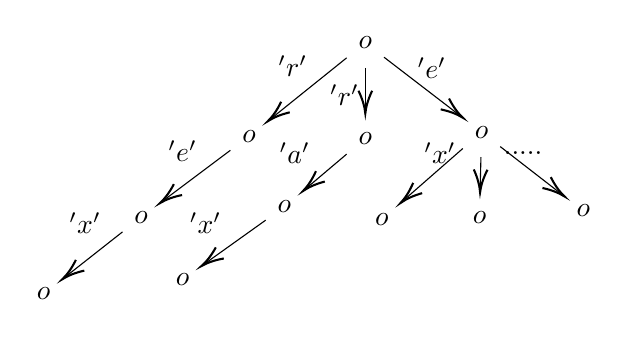
\begin{tikzpicture}[x=0.75pt,y=0.75pt,yscale=-1,xscale=1]
    %uncomment if require: \path (0,235); %set diagram left start at 0, and has height of 235
    
    
    % Text Node
    \draw (154,44) node    {$o$};
    % Text Node
    \draw (98,89) node    {$o$};
    % Text Node
    \draw (119,55) node    {$'r'$};
    % Text Node
    \draw (154,90) node    {$o$};
    % Text Node
    \draw (210,87) node    {$o$};
    % Text Node
    \draw (144,69) node    {$'r'$};
    % Text Node
    \draw (186,56) node    {$'e'$};
    % Text Node
    \draw (66,96) node    {$'e'$};
    % Text Node
    \draw (46,128) node    {$o$};
    % Text Node
    \draw (-1,165) node    {$o$};
    % Text Node
    \draw (19,131) node    {$'x'$};
    \draw (77,131) node    {$'x'$};
    % Text Node
    \draw (115,123) node    {$o$};
    % Text Node
    \draw (120,97) node    {$'a'$};
    \draw (190,97) node    {$'x'$};
    \draw (230,97) node    {$.....$};
    % Text Node
    \draw (66,158) node    {$o$};
    % Text Node
    \draw (162,129) node    {$o$};
    % Text Node
    \draw (209,128) node    {$o$};
    % Text Node
    \draw (259,125) node    {$o$};
    % Connection
    \draw    (145,51.23) -- (108.56,80.52) ;
    \draw [shift={(107,81.77)}, rotate = 321.22] [color={rgb, 255:red, 0; green, 0; blue, 0 }  ][line width=0.75]    (10.93,-3.29) .. controls (6.95,-1.4) and (3.31,-0.3) .. (0,0) .. controls (3.31,0.3) and (6.95,1.4) .. (10.93,3.29)   ;
    % Connection
    \draw    (154,56) -- (154,76) ;
    \draw [shift={(154,78)}, rotate = 270] [color={rgb, 255:red, 0; green, 0; blue, 0 }  ][line width=0.75]    (10.93,-3.29) .. controls (6.95,-1.4) and (3.31,-0.3) .. (0,0) .. controls (3.31,0.3) and (6.95,1.4) .. (10.93,3.29)   ;
    % Connection
    \draw    (163,50.91) -- (199.41,78.87) ;
    \draw [shift={(201,80.09)}, rotate = 217.52] [color={rgb, 255:red, 0; green, 0; blue, 0 }  ][line width=0.75]    (10.93,-3.29) .. controls (6.95,-1.4) and (3.31,-0.3) .. (0,0) .. controls (3.31,0.3) and (6.95,1.4) .. (10.93,3.29)   ;
    % Connection
    \draw    (89,95.75) -- (56.6,120.05) ;
    \draw [shift={(55,121.25)}, rotate = 323.13] [color={rgb, 255:red, 0; green, 0; blue, 0 }  ][line width=0.75]    (10.93,-3.29) .. controls (6.95,-1.4) and (3.31,-0.3) .. (0,0) .. controls (3.31,0.3) and (6.95,1.4) .. (10.93,3.29)   ;
    % Connection
    \draw    (37,135.09) -- (9.57,156.68) ;
    \draw [shift={(8,157.91)}, rotate = 321.78999999999996] [color={rgb, 255:red, 0; green, 0; blue, 0 }  ][line width=0.75]    (10.93,-3.29) .. controls (6.95,-1.4) and (3.31,-0.3) .. (0,0) .. controls (3.31,0.3) and (6.95,1.4) .. (10.93,3.29)   ;
    % Connection
    \draw    (145,97.62) -- (125.53,114.09) ;
    \draw [shift={(124,115.38)}, rotate = 319.76] [color={rgb, 255:red, 0; green, 0; blue, 0 }  ][line width=0.75]    (10.93,-3.29) .. controls (6.95,-1.4) and (3.31,-0.3) .. (0,0) .. controls (3.31,0.3) and (6.95,1.4) .. (10.93,3.29)   ;
    % Connection
    \draw    (106,129.43) -- (76.63,150.41) ;
    \draw [shift={(75,151.57)}, rotate = 324.46000000000004] [color={rgb, 255:red, 0; green, 0; blue, 0 }  ][line width=0.75]    (10.93,-3.29) .. controls (6.95,-1.4) and (3.31,-0.3) .. (0,0) .. controls (3.31,0.3) and (6.95,1.4) .. (10.93,3.29)   ;
    % Connection
    \draw    (201,94.88) -- (172.51,119.81) ;
    \draw [shift={(171,121.13)}, rotate = 318.81] [color={rgb, 255:red, 0; green, 0; blue, 0 }  ][line width=0.75]    (10.93,-3.29) .. controls (6.95,-1.4) and (3.31,-0.3) .. (0,0) .. controls (3.31,0.3) and (6.95,1.4) .. (10.93,3.29)   ;
    % Connection
    \draw    (209.71,99) -- (209.34,114) ;
    \draw [shift={(209.29,116)}, rotate = 271.4] [color={rgb, 255:red, 0; green, 0; blue, 0 }  ][line width=0.75]    (10.93,-3.29) .. controls (6.95,-1.4) and (3.31,-0.3) .. (0,0) .. controls (3.31,0.3) and (6.95,1.4) .. (10.93,3.29)   ;
    % Connection
    \draw    (219,93.98) -- (248.42,116.79) ;
    \draw [shift={(250,118.02)}, rotate = 217.79] [color={rgb, 255:red, 0; green, 0; blue, 0 }  ][line width=0.75]    (10.93,-3.29) .. controls (6.95,-1.4) and (3.31,-0.3) .. (0,0) .. controls (3.31,0.3) and (6.95,1.4) .. (10.93,3.29)   ;
    
    \end{tikzpicture}
    

    By using prefix trees, searching and matching can be done without traversing the entire array, and the time complexity is reduced to $O(E[strlen])$. In the implementation, a prefix tree can be created for all instruction operator names and register names before executing the CPU instruction cycle, so that the matching time can be reduced during the execution of the instruction cycle. Each node of the prefix tree usually includes a char$\rightarrow$(void *) mapped data structure, where char is the character and (void *) is the address of the subtree. As you can see, the prefix tree is very similar to the DFA, except that the prefix tree automatically builds the state transfer (so it is not streamlined enough), while the DFA requires us to calculate the state transfer in advance.
\subsection{Examples of accepting yml}
We cannot do it, because of indent can only be accepted with stack machine.

    \begin{lstlisting}[language={[ANSI]C},
            numbers=left,
            numberstyle=\extratiny,
            basicstyle=\small]
// Identity definitions
<whitespace> ::= " " | "\t"
<in-line-whitespace> ::= <whitespace> | <whitespace> <in-line-whitespace>
<digit> ::= "0" | "1" | "2" | "3" | "4" | "5" | "6" | "7" | "8" | "9"
<integer-number> ::= <digit> | <digit> <integer-number>
<end-of-line> ::= "\r\n" | "\r" | "\n"
<non-whitespace> ::=
<non-whitespace-word> ::= <non-whitespace> | <non-whitespace> <non-whitespace-word>

// Basic document structure
<yaml-stream> ::= <yaml-document-list>
<yaml-document-list> ::= <yaml-document> | <yaml-document> <yaml-document-list>
<yaml-document> ::= <yaml-directive-list> <yaml-directives-end> <yaml-content-list>
        <yaml-document-end>
<yaml-directive-list> ::= <yaml-directive> <yaml-directive-list> | ""
<yaml-directive> ::= <yaml-directive-yaml> | <yaml-directive-tag>
<yaml-directive-yaml> ::= "%YAML" <in-line-whitespace> <integer-number> "." <integer-number>
         <end-of-line> | ""
<yaml-directive-tag> ::= "%TAG" <in-line-whitespace> <yaml-tag-handle> <in-line-whitespace> 
        <yaml-tag-prefix> <end-of-line> <yaml-directive-tag> | ""
<yaml-tag-handle> ::= "!" | "!!" | "!" <non-whitespace-word> "!"
<yaml-tag-prefix> ::= "!" <non-whitespace-word> | <non-whitespace-word>
<yaml-directives-end> ::= "---" | ""
<yaml-content-list> ::= <yaml-content> <yaml-content-list> | <yaml-content> <end-of-line>
<yaml-document-end> ::= "..." | ""

// Internals of an individual document
<yaml-content> ::=
    \end{lstlisting}

\subsection{What language is accepted by the following DFA?}
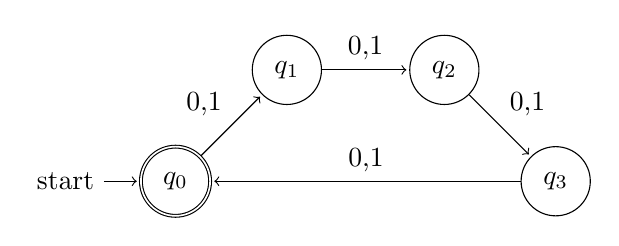
\begin{tikzpicture}[shorten >=1pt,node distance=2cm,on grid,auto]
    \node[state,initial,accepting] (q_0)   {$q_0$};
    \node[state] (q_1) [above right=of q_0] {$q_1$};
    \node[state] (q_2) [right=of q_1] {$q_2$};
    \node[state] (q_3) [below right=of q_2] {$q_3$};
    \path[->]
    (q_0) edge  node {0,1} (q_1)
    (q_1) edge  node  {0,1} (q_2)
    (q_2) edge  node  {0,1} (q_3)
    (q_3)edge  node  [above]{0,1} (q_0);

\end{tikzpicture}
\\
\textbf{Answer:}

\subsection{What language is accepted by the following NFA?}
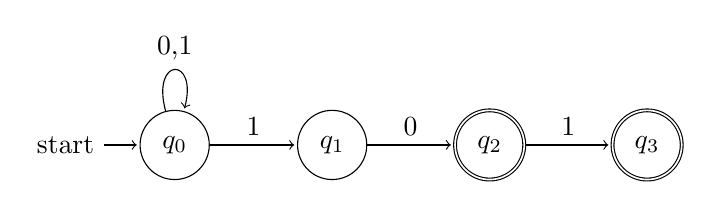
\begin{tikzpicture}[shorten >=1pt,node distance=2cm,on grid,auto]
    \node[state,initial] (q_0)   {$q_0$};
    \node[state] (q_1) [ right=of q_0] {$q_1$};
    \node[state,accepting] (q_2) [right=of q_1] {$q_2$};
    \node[state,accepting] (q_3) [ right=of q_2] {$q_3$};
    \path[->]
    (q_0) edge [loop above] node {0,1} ()
        edge  node  [above]{1} (q_1)
    (q_1) edge  node  {0} (q_2)
    (q_2) edge  node  {1} (q_3);

\end{tikzpicture}
\\
\textbf{Answer:}

\subsection{What language is accepted by the following NFA?}
\begin{tikzpicture}[shorten >=1pt,node distance=2cm,on grid,auto]
    \node[state,initial,accepting] (q_0)   {$q_0$};
    \node[state] (q_3) [ right=of q_2] {$q_3$};
    \node[state,accepting] (q_2) [right=of q_1] {$q_2$};
    \node[state,accepting] (q_1) [ right=of q_0] {$q_1$};
    \node[state,accepting] (q_4) [ right=of q_3] {$q_4$};
    \node[state,accepting] (q_5) [ right=of q_4] {$q_5$};
    \path[->]
    (q_0) 
        edge  node  [above]{0,1} (q_1)
    (q_1) edge  node  {0,1} (q_2)
    (q_2) edge  node  {0,1} (q_3)
    (q_3) edge  node  {0,1} (q_4)
    (q_4) edge  node  {0,1} (q_5)
    (q_5) edge [loop above] node {0,1} ();
\end{tikzpicture}
\\
\textbf{Answer:}


\subsection{Construct the NFA that accepts}
\subsubsection{$x(zy?|(yz)*)$}
\textbf{Answer:}
\subsubsection{$(10)*1*01*0$}
\textbf{Answer:}

\subsection{Minimized the NFA}
  \begin{enumerate}
	\item Original NFA, $\Sigma = \{a, b, c\}$:
	\\
	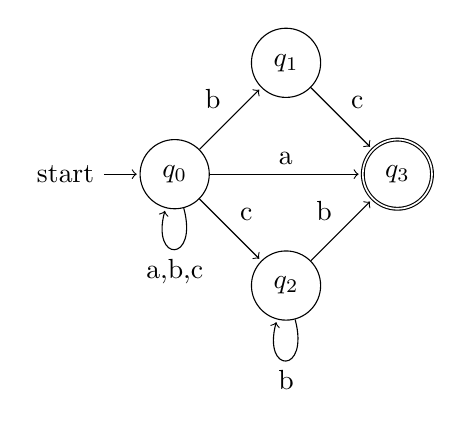
\begin{tikzpicture}[shorten >=1pt,node distance=2cm,on grid,auto]
		\node[state,initial] (q_0)   {$q_0$};
		\node[state] (q_1) [above right=of q_0] {$q_1$};
		\node[state] (q_2) [below right=of q_0] {$q_2$};
		\node[state,accepting](q_3) [below right=of q_1] {$q_3$};
		\path[->]
		(q_0) edge [loop below] node {a,b,c} ()
			  edge  node  [above] {a} (q_3)
			  edge  node  {b} (q_1)
			  edge  node  {c} (q_2)
		(q_1) edge  node  {c} (q_3)
		(q_2) edge  node  {b} (q_3)
			  edge  [loop below] node  {b} ();
	\end{tikzpicture}

\textbf{Answer:}
$
\\
\\
\\
\\
\\
$
\section{Pumpingg Lemma}
Pumping Lemma: For any DFA (or NFA or regular expression) that accepts an
infinite number of strings, there is some minimum length, \(M,\) such that any string
with length greater than or equal to \(M\) that the machine accepts must have the form
\(u x v,\) where \(u, x,\) and \(v\) are strings, \(x\) is not empty, the length of \(u x\) is \(\leq M,\) and the
machine accepts all strings of the form \(u x^{n} v,\) for all \(n \geq 0\).
\subsection{Proof of not regular} Let \(A=\left\{1^{j} z \mid z \in\{0,1\}^{*}\right.\) and \(z\) contains at most \(j\) i's, for any \(\left.j \geq 1\right\} .\) Prove, by the
pumping lemma, that \(A\) is not regular.\\
\textbf{Answer:}
$
\\
\\
\\
\\
\\
$


\end{document}
